\newsection{3}{Applications of First Order Equations} {Elementary Mechanics}
\currentpdfbookmark{Section 4.3 Elementary Mechanics}{section:4.3}
\vskip14pt
\renewcommand{\thissection}{\sectiontitle{\,
ELEMENTARY MECHANICS}}
\thissection

\boxit{Newton's Second Law of Motion}

\noindent
In this section we consider an object with constant mass $m$ moving
along a line under a force $F$. Let $y=y(t)$ be the displacement of
the object from a reference point on the line at time $t$, and let
$v=v(t)$ and $a=a(t)$ be the velocity and acceleration of the object
at time $t$. Thus, $v=y'$ and $a=v'=y''$, where the prime denotes
differentiation with respect to $t$. Newton's second law of motion
asserts that the force $F$ and the acceleration $a$ are related by the
equation
\begin{equation} \label{eq:4.3.1}
F=ma.
\end{equation}

\boxit{Units}

\noindent
In applications there are three main sets of units in use for length,
mass, force, and time: the cgs, mks, and British systems. All three
use the second as the unit of time. Table~1 shows the other units.
 Consistent with (\ref{eq:4.3.1}), the unit of
force in each system is defined to be the force required to impart an
acceleration of (one unit of length)$/s^2$ to one unit of
mass.

\bigskip
\begin{center}
\begin{tabular}{|c|c|c|c|}
\hline
& {\bf Length}&{\bf Force}& {\bf Mass}\\\hline
  cgs & centimeter (cm) & dyne (d) & gram (g)\\\hline
 mks & meter (m) & newton (N) & kilogram (kg) \\\hline
British & foot (ft) & pound (lb) & slug (sl)\\\hline
\end{tabular}

\medskip
Table 1.
\end{center}

If we assume that Earth is a perfect sphere with constant mass
density,  Newton's law of gravitation (discussed later in this
section) asserts that the force exerted on an object by Earth's
gravitational field is proportional to the mass of the object and
inversely proportional to the square of its  distance from the
center of Earth. However, if the object remains sufficiently close to
Earth's surface, we may assume that the gravitational force is
constant and equal to its value at the surface. The magnitude of this
force is $mg$, where $g$ is called the {\color{blue}\it acceleration due to
gravity}. (To be completely accurate, $g$ should be called the {\color{blue}\it
magnitude of the acceleration due to gravity at Earth's surface}.)\
This quantity has been determined experimentally. Approximate
values of $g$  are
$$\begin{array}{rl}
g &=980\ \mbox{cm/s}^2 \hskip40pt \mbox{(cgs)}   \\
g &=9.8\ \mbox{m/s}^2 \hskip48pt \mbox{(mks)}   \\
g &=32\ \mbox{ft/s}^2 \hskip52pt \mbox{(British)}.
\end{array}$$

In general, the force $F$ in (\ref{eq:4.3.1}) may depend upon $t$, $y$, and
$y'$. Since $a=y''$,  (\ref{eq:4.3.1}) can be written in the
form
\begin{equation} \label{eq:4.3.2}
my''=F(t,y,y'),
\end{equation}
which is a second order equation. We'll consider this equation with
restrictions on $F$ later;     however, since Chapter~2
dealt only with first order equations, we consider here only problems in
which (\ref{eq:4.3.2}) can be recast as a first order equation. This is
possible if $F$ does not depend on $y$, so (\ref{eq:4.3.2}) is of the form
$$
my''=F(t,y').
$$
 Letting $v=y'$ and $v'=y''$ yields a first order
equation for $v$:
\begin{equation} \label{eq:4.3.3}
mv'=F(t,v).
\end{equation}
Solving this equation yields $v$ as a function of $t$. If we know
$y(t_0)$ for some time $t_0$, we can  integrate $v$ to obtain $y$
as a function of $t$.

Equations of the form (\ref{eq:4.3.3}) occur in problems involving motion
through a resisting medium.

\boxit{Motion Through a Resisting Medium Under Constant
Gravitational Force}

\noindent
Now we consider an object moving vertically in some medium. We assume
that the only forces acting on the object are gravity and resistance
from the medium. We also assume that the motion takes place close to
Earth's surface and take the upward direction to be positive, so
 the gravitational force can be assumed to have the constant value
 $-mg$. We'll see that, under reasonable assumptions on the
resisting force, the velocity approaches a limit as $t\to\infty$.
We call this limit the {\color{blue}\it terminal velocity\/}.

\begin{example}\label{example:4.3.1} \rm
An object with mass $m$ moves under constant gravitational force
through a medium that exerts a resistance with magnitude proportional
to the speed of the object. (Recall that the speed of an object is
$|v|$, the absolute value of its velocity $v$.) Find the velocity of
the object as a function of $t$, and find the terminal velocity.
Assume  that the initial velocity is $v_0$.
 \end{example}

\solution
The total force acting on the object is
\begin{equation} \label{eq:4.3.4}
F=-mg+F_1,
\end{equation}
where $-mg$ is  the force due to  gravity and $F_1$ is the
resisting force of the medium, which has magnitude $k|v|$, where $k$ is a
positive constant. If the
object is moving downward ($v\le 0$),  the resisting force is
upward (Figure~\ref{figure:4.3.1}\part{a}), so
$$
F_1=k|v|=k(-v)=-kv.
$$
On the other hand, if the object is moving upward ($v\ge 0$),
the resisting force is downward (Figure~\ref{figure:4.3.1}\part{b}), so
$$
F_1=-k|v|=-kv.
$$
Thus, (\ref{eq:4.3.4}) can be written as
\begin{equation} \label{eq:4.3.5}
F=-mg-kv,
\end{equation}
regardless of the sign of the velocity.

\begin{figure}[tbp]
  \centering
  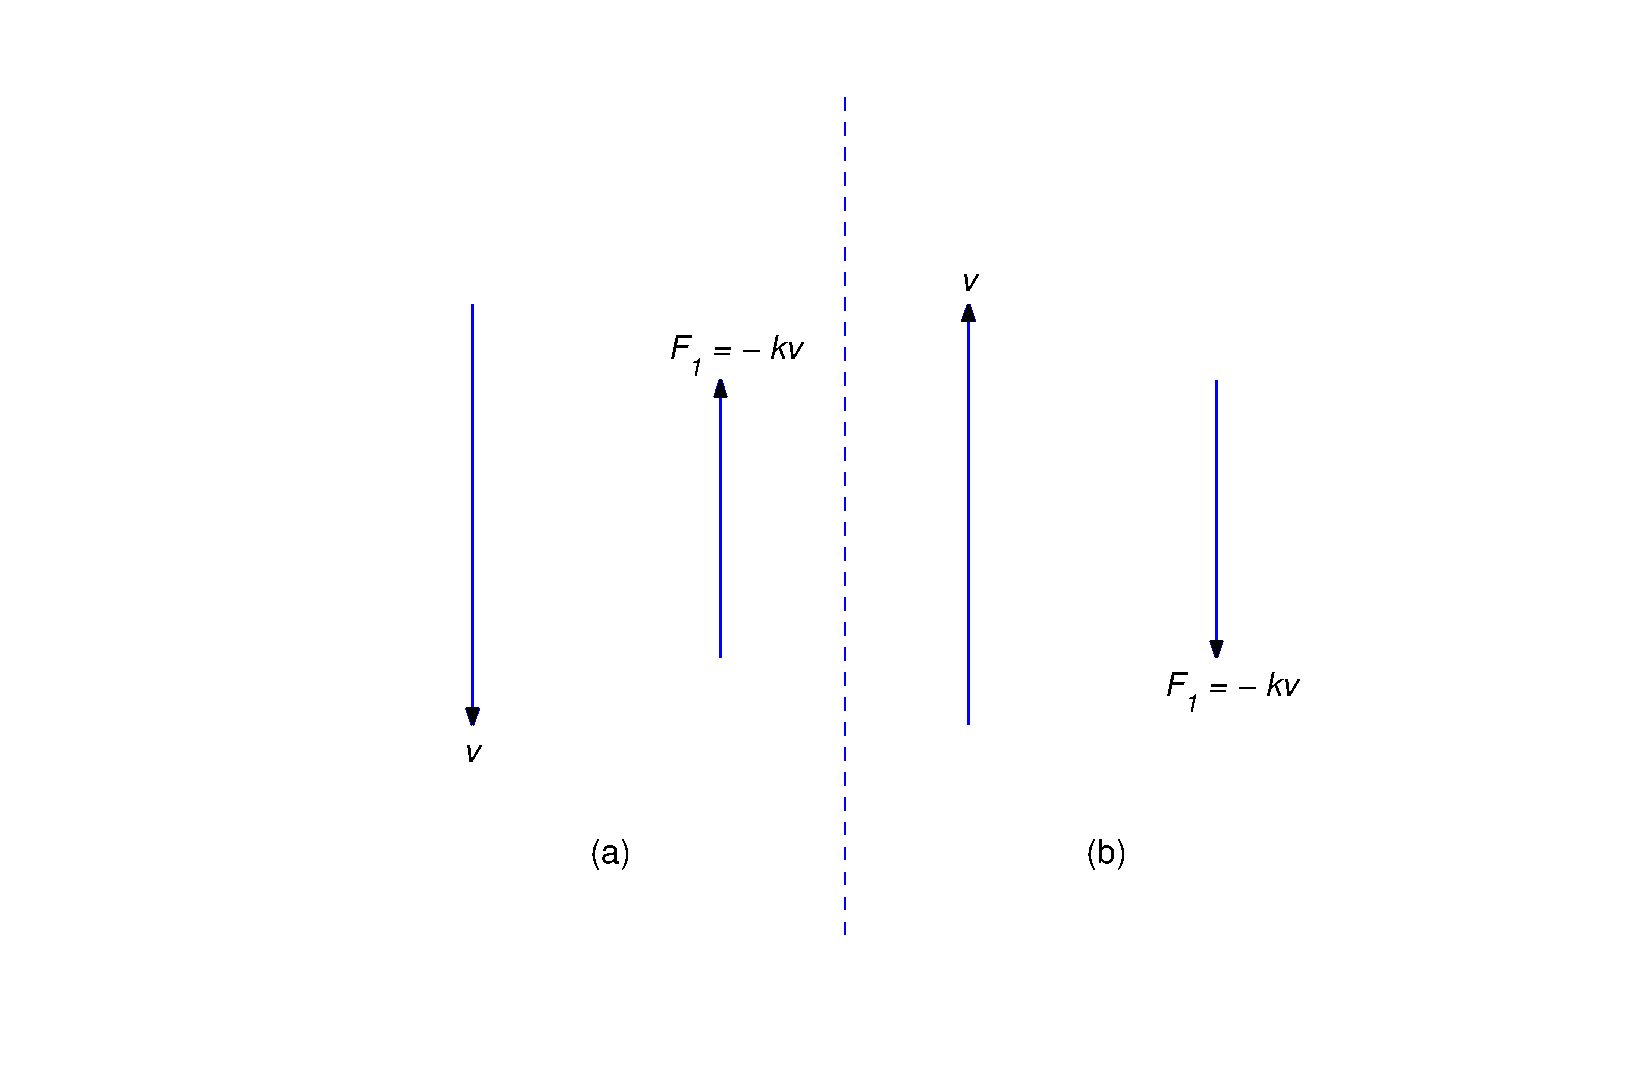
\includegraphics[bb=-78 148 689 643,width=5.67in,height=3.66in,keepaspectratio]{fig040301}
\color{blue}
  \caption{Resistive forces}
  \label{figure:4.3.1}
\end{figure}

From Newton's second law of motion,
$$
F=ma=mv',
$$
 so (\ref{eq:4.3.5}) yields
$$
mv'=-mg-kv,
$$
 or
\begin{equation} \label{eq:4.3.6}
v'+{k\over m}v=-g.
\end{equation}
Since $e^{-kt/m}$ is a solution of the  complementary
equation, the solutions of (\ref{eq:4.3.6}) are of the form
$v=ue^{-kt/m}$, where $u'e^{-kt/m}=-g$, so $u'=-ge^{kt/m}$.
Hence,
$$
u=-{mg\over k} e^{kt/m}+c,
$$
so
\begin{equation} \label{eq:4.3.7}
v=ue^{-kt/m}=-{mg\over k}+ce^{-kt/m}.
\end{equation}
Since
 $v(0)=v_0$,
$$
v_0=-{mg\over k}+c,
$$
 so
$$
c=v_0+{mg\over k}
$$
 and (\ref{eq:4.3.7}) becomes
$$
v=-{mg\over k}+\left(v_0+{mg\over k}\right) e^{-kt/m}.
$$
Letting $t\to\infty$ here shows that the terminal velocity is
$$
\lim_{t\to\infty} v(t)=-{mg\over k},
$$
which  is independent of the
initial velocity $v_0$ (Figure~\ref{figure:4.3.2}).

\begin{figure}[tbp]
  \centering
  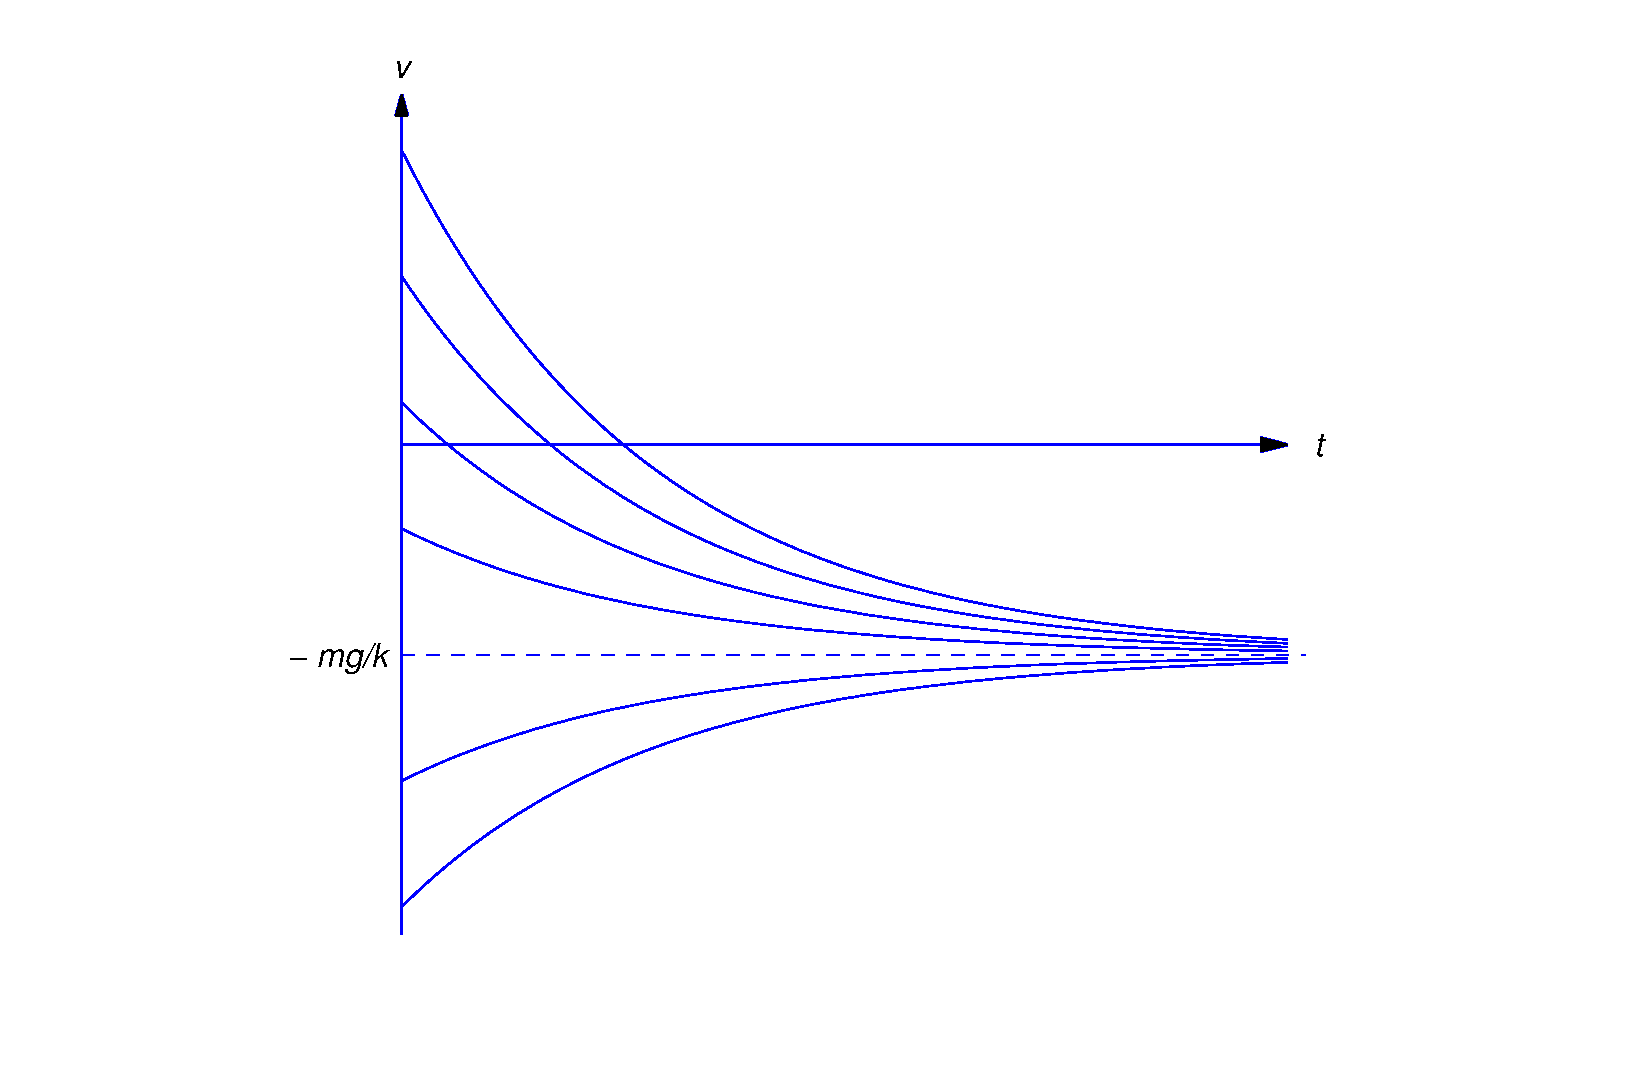
\includegraphics[bb=-78 148 689 643,width=5.67in,height=3.66in,keepaspectratio]{fig040302}
\color{blue}
  \caption{Solutions of $mv'=-mg-kv$}
  \label{figure:4.3.2}
\end{figure}

\begin{example}\label{example:4.3.2} \rm
A 960-lb object is given an initial upward velocity of 60 ft/s near
the surface of Earth. The atmosphere resists the motion with a force
of 3 lb for each ft/s of speed. Assuming that the only other force
acting on the object is constant gravity, find its velocity $v$ as a
function of $t$, and find its  terminal velocity.
\end{example}

\solution
Since $mg=960$ and $g=32$,   $m=960/32=30$.  The atmospheric
resistance is $-3v$  lb if $v$ is expressed in feet
per second.  Therefore
$$
30v'=-960-3v,
$$
which we rewrite as
$$
v'+{1\over 10}v=-32.
$$
Since $e^{-t/10}$ is a solution of the complementary equation, the
solutions of this equation are of the form $v=ue^{-t/10}$, where
$u'e^{-t/10}=-32$, so $u'=-32e^{t/10}$. Hence,
$$
u=-320 e^{t/10}+c,
$$
so
\begin{equation} \label{eq:4.3.8}
v=ue^{-t/10}=-320+ce^{-t/10}.
\end{equation}
The initial velocity is 60 ft/s in the upward (positive) direction;
hence, $v_0=60$. Substituting $t=0$ and $v=60$ in (\ref{eq:4.3.8})
yields
$$
60=-320+c,
$$
 so $c=380$, and (\ref{eq:4.3.8}) becomes
$$
v=-320+380e^{-t/10}\ \mbox{ft/s}
$$
The terminal velocity is
$$
\lim_{t\to\infty}v(t)=-320\mbox{ ft/s.}
$$

\begin{example}\label{example:4.3.3} \rm
A 10 kg mass is given an initial velocity $v_0\le0$
 near Earth's surface. The only forces acting on it are
gravity and atmospheric resistance proportional to the square of the
speed. Assuming that the resistance is 8 N if the speed is 2 m/s,
find the velocity of the object as a function of $t$, and
find the terminal velocity.
\end{example}

\solution Since the object is falling, the resistance is in the upward
(positive) direction. Hence,
\begin{equation} \label{eq:4.3.9}
mv'=-mg+kv^2,
\end{equation}
where $k$ is a constant. Since the magnitude of the resistance is 8 N
when $v=2$ m/s,
$$
k(2^2)=8,
$$
 so $k=2\  \mbox{N-s}^2/\mbox{m}^2$.  Since
$m=10$ and $g=9.8$, (\ref{eq:4.3.9}) becomes
\begin{equation} \label{eq:4.3.10}
10v'=-98+2v^2=2(v^2-49).
\end{equation}
If $v_0=-7$, then $v\equiv-7$ for all $t\ge0$. If $v_0\ne-7$,
we separate  variables to obtain
\begin{equation} \label{eq:4.3.11}
{1\over v^2-49}v'={1\over5},
\end{equation}
which is convenient for the required partial fraction expansion
\begin{equation} \label{eq:4.3.12}
\frac{1}{v^2-49} =\frac{1}{(v-7)(v+7)}
={1\over 14}\left[{1\over v-7}
-{1\over v+7}\right].
\end{equation}
 Substituting (\ref{eq:4.3.12})  into (\ref{eq:4.3.11}) yields
$$
{1\over14}\left[{1\over v-7}-{1\over v+7}\right]v'={1\over5},
$$
 so
$$
\left[{1\over v-7}-{1\over v+7}\right]v'={14\over5}.
$$
Integrating this yields
$$
\ln |v-7|-\ln|v+7|=14t/5+k.
$$
Therefore
$$
\left|{v-7\over v+7}\right|=e^ke^{14t/5}.
$$
Since  Theorem~\ref{thmtype:2.3.1}  implies  that  $(v-7)/(v+7)$   can't
change sign (why?), we can rewrite the last equation as
 \begin{equation} \label{eq:4.3.13}
 {v-7\over v+7}=ce^{14t/5},
\end{equation}
which is an implicit solution of (\ref{eq:4.3.10}).
Solving this for $v$ yields
\begin{equation} \label{eq:4.3.14}
v=-7{c+e^{-14t/5}\over c-e^{-14t/5}}.
\end{equation}
 Since $v(0)=v_0$, it
 (\ref{eq:4.3.13}) implies that
$$
c={v_0-7\over v_0+7}.
$$
 Substituting this into (\ref{eq:4.3.14}) and simplifying yields
$$
v=-7{v_0(1+e^{-14t/5})-7(1-e^{-14t/5})\over
v_0(1-e^{-14t/5})-7(1+e^{-14t/5}}.
$$
Since $v_0\le0$, $v$ is defined and negative for all
$t>0$. The terminal velocity is
$$
\lim_{t\to\infty} v(t)=-7\  \mbox{m/s},
$$
independent of $v_0$. More generally, it
can be shown (Exercise~\ref{exer:4.3.11}) that if $v$ is any solution
of (\ref{eq:4.3.9}) such that $v_0\le0$ then
$$
\lim_{t\to\infty}v(t)=-\sqrt{mg\over k}
$$
(Figure~\ref{figure:4.3.3}).

      \begin{figure}[tbp]
  \centering
  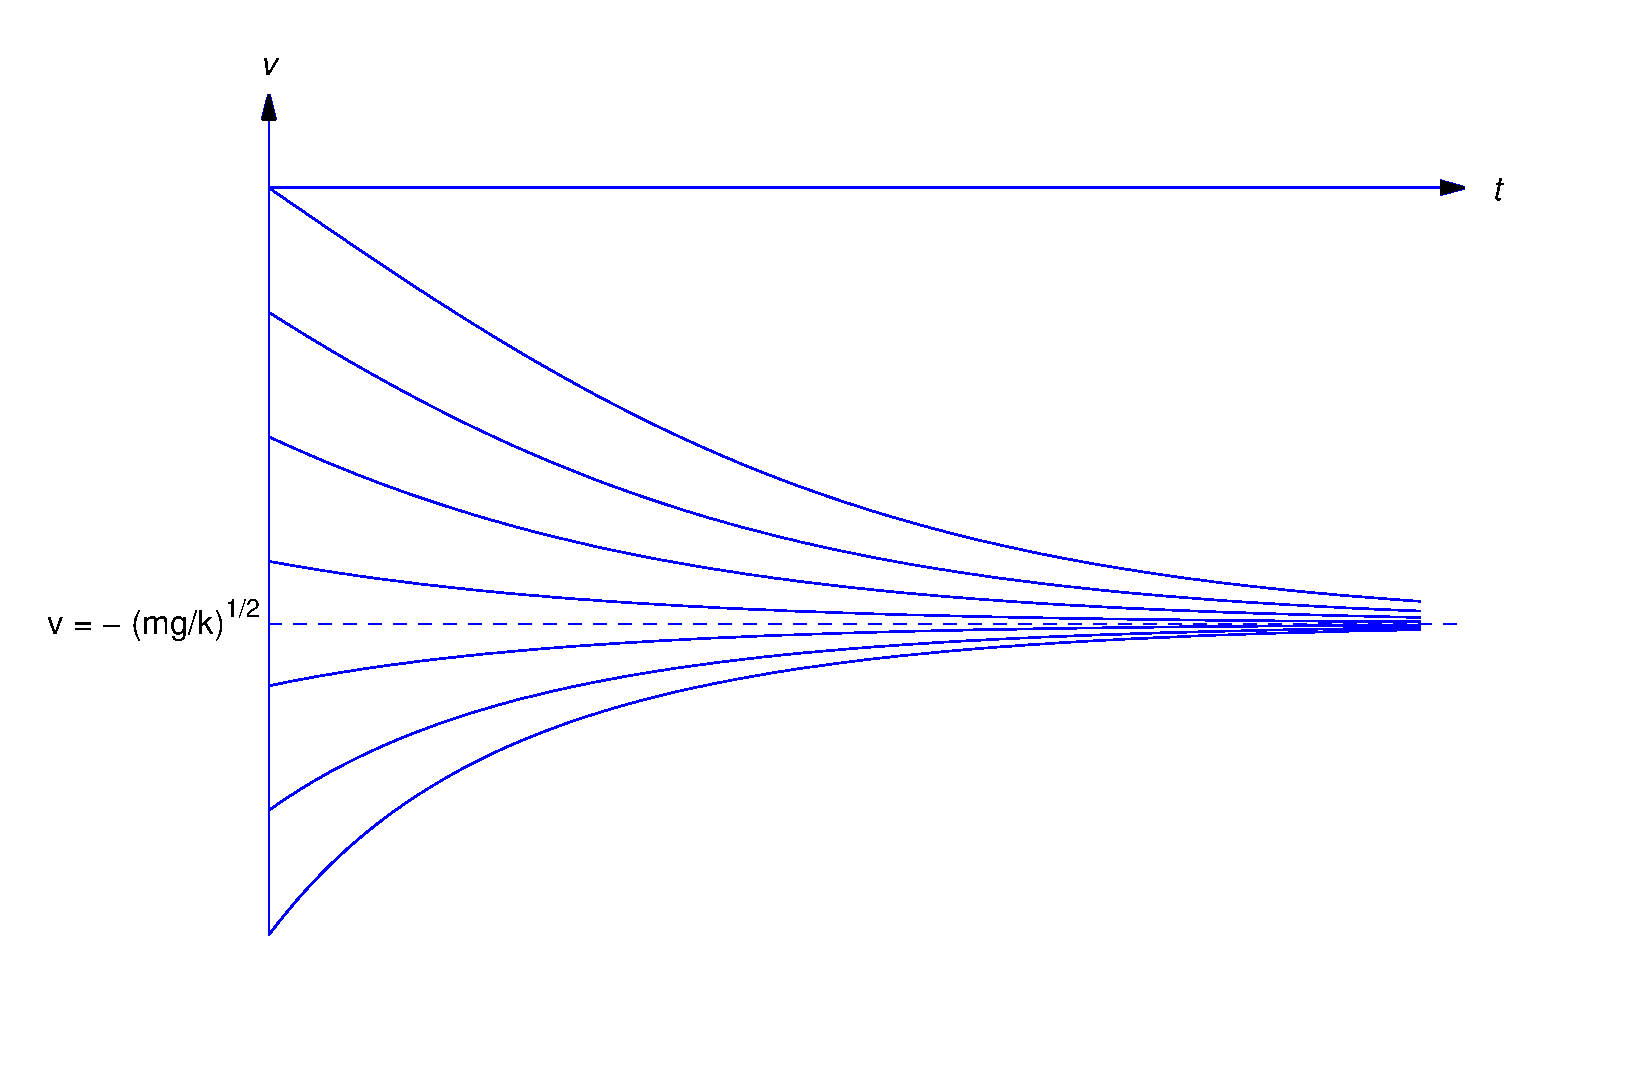
\includegraphics[bb=-78 148 689 643,width=5.67in,height=3.66in,keepaspectratio]{fig040303}
\color{blue}
  \caption{Solutions of $mv'=-mg+kv^2,\ v(0)=v_0\le0$}
  \label{figure:4.3.3}
\end{figure}

\begin{example}\label{example:4.3.4} \rm
A 10-kg mass is launched vertically upward from Earth's surface with
an initial velocity of $v_0$ m/s. The only forces acting on the mass
are gravity and atmospheric resistance proportional to the square of
the speed. Assuming that the atmospheric resistance is 8 N if the
speed is 2 m/s, find the time $T$ required for the mass to reach
maximum altitude.
\end{example}

\solution  The mass will
climb while $v>0 $ and reach its maximum altitude when $v=0$.
Therefore $v>0$ for $0\le t<T$ and $v(T)=0$. Although the mass of
the object and our assumptions concerning the forces acting on it are
the same as those in Example 3,  (\ref{eq:4.3.10}) does
not apply here, since the resisting force is negative if $v>0$;
therefore, we replace (\ref{eq:4.3.10}) by
\begin{equation} \label{eq:4.3.15}
10v'=-98-2v^2.
\end{equation}

Separating variables  yields
$$
{5\over v^2+49}v'=-1,
$$
 and integrating this yields
$$
{5\over7}\tan^{-1}{v\over7}=-t+c.
$$
 (Recall that $\tan^{-1}u$ is the number $\theta$
such that $-\pi/2 < \theta < \pi/2$ and $\tan \theta=u$.)
 Since $v(0)=v_0$,
$$
c={5\over7}\tan^{-1}{v_0\over7},
$$
so $v$ is defined implicitly by
\begin{equation} \label{eq:4.3.16}
{5\over7} \tan^{-1}{v\over7}=-t+{5\over7}
\tan^{-1}{v_0\over7}, \quad 0\le t\le T.
\end{equation}
Solving this for $v$ yields
\begin{equation} \label{eq:4.3.17}
v=7\tan\left(-{7t\over5}+\tan^{-1}{v_0\over7}\right).
\end{equation}
Using the identity
$$
\tan(A-B)={\tan A-\tan B\over1+\tan A\tan B}
$$
with $A=\tan^{-1}(v_0/7)$ and $B=7t/5$, and noting that
$\tan(\tan^{-1}\theta)=\theta$,
we can simplify (\ref{eq:4.3.17}) to
$$
v=7{v_0-7\tan(7t/5)\over7+v_0\tan(7t/5)}.
$$

 Since $v(T)=0$ and $\tan^{-1}(0)=0$, (\ref{eq:4.3.16}) implies that
$$
-T+{5\over7} \tan^{-1}{v_0\over7}=0.
$$
Therefore
$$
T={5\over7} \tan^{-1}{v_0\over7}.
$$
Since $\tan^{-1}(v_0/7)<\pi/2$ for all $v_0$,
the  time required for the mass to reach its maximum
altitude is less than
$$
{5\pi\over 14} \approx 1.122\  \mbox{s}
$$
regardless of the initial velocity.  Figure~\ref{figure:4.3.4}
shows graphs of $v$ over $[0,T]$ for various values of $v_0$.

\begin{figure}[tbp]
  \centering
  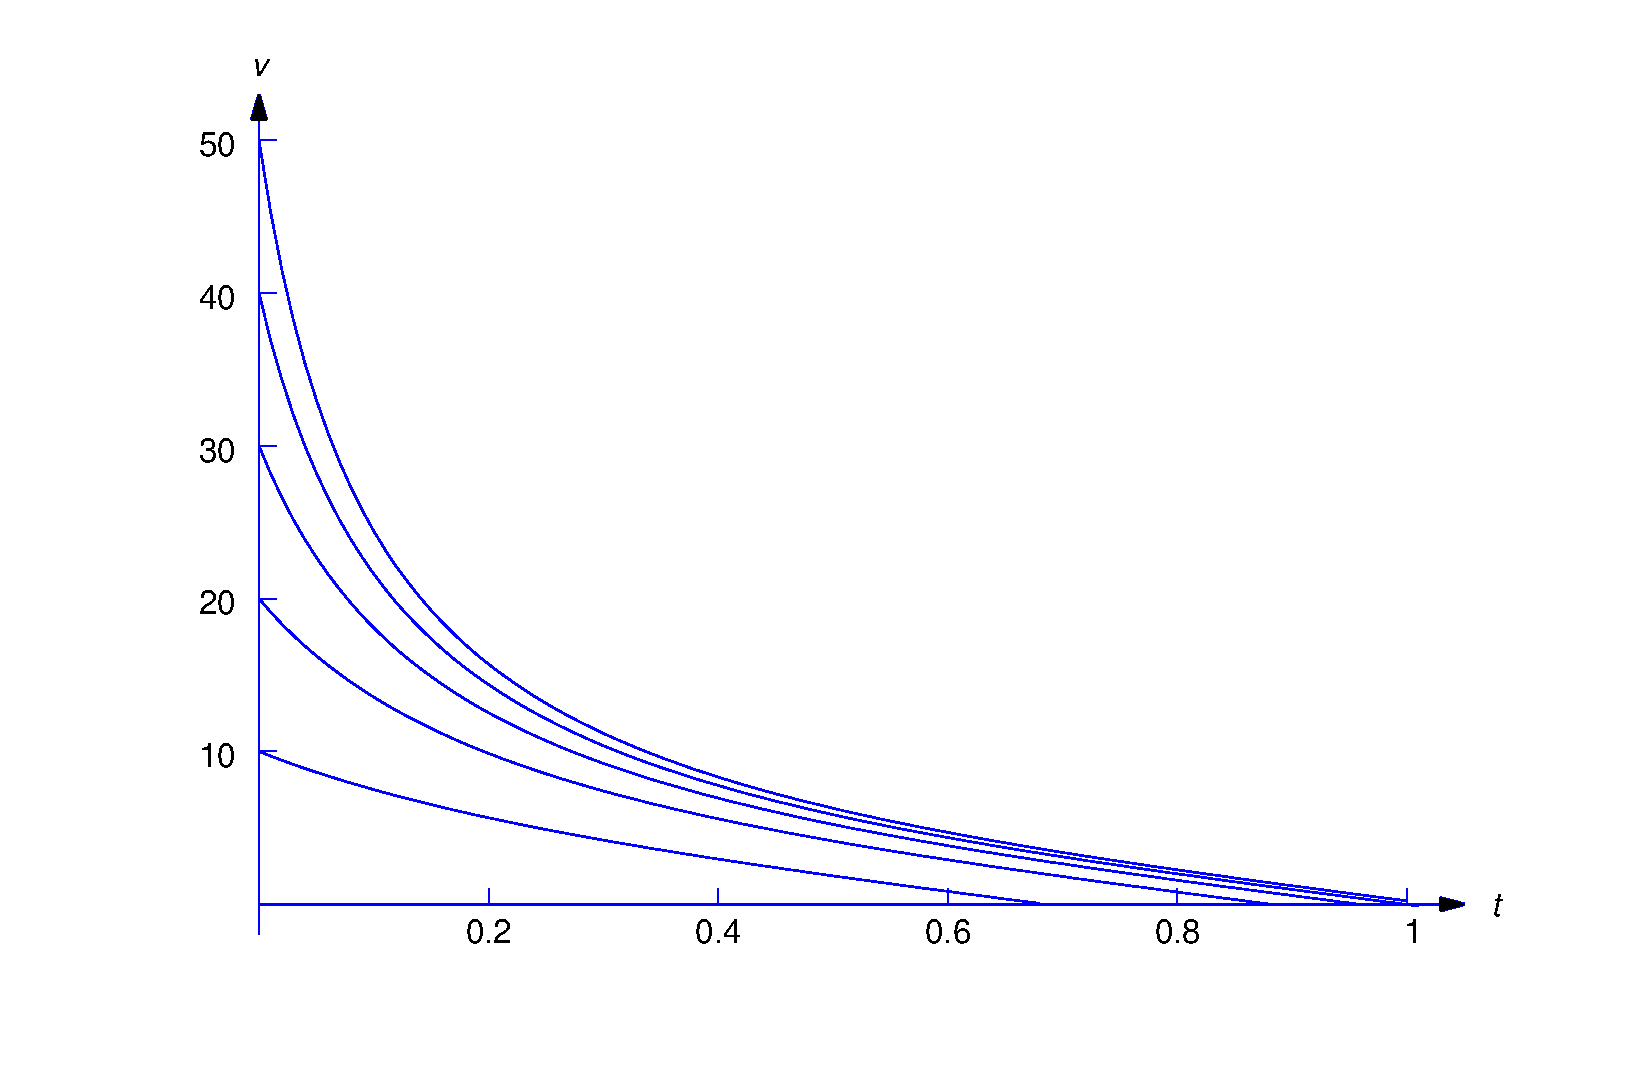
\includegraphics[bb=-78 148 689 643,width=5.67in,height=3.66in,keepaspectratio]{fig040304}
\color{blue}
\caption{Solutions of (\ref{eq:4.3.15}) for various
$v_0>0$}
  \label{figure:4.3.4}
\end{figure}

\newpage

\boxit{Escape Velocity}

\noindent
Suppose a space vehicle is launched vertically and its fuel is
exhausted when the vehicle reaches an altitude $h$ above Earth, where
$h$ is sufficiently large so that resistance due to Earth's atmosphere
can be neglected. Let $t=0$ be the time when burnout occurs.
Assuming that the gravitational forces of all other celestial bodies
can be neglected, the motion of the vehicle for $t > 0$ is that of an
object with constant mass $m$ under the influence of Earth's
gravitational force, which we now assume to vary inversely with the
square of the distance from Earth's center;  thus, if we take the
upward direction to be positive then
gravitational force on the vehicle at an altitude $y$ above Earth is
\begin{equation} \label{eq:4.3.18}
F=-{K\over(y+R)^2},
\end{equation}
where $R$ is  Earth's radius (Figure~\ref{figure:4.3.5}).

\begin{figure}[tbp]
  \centering
  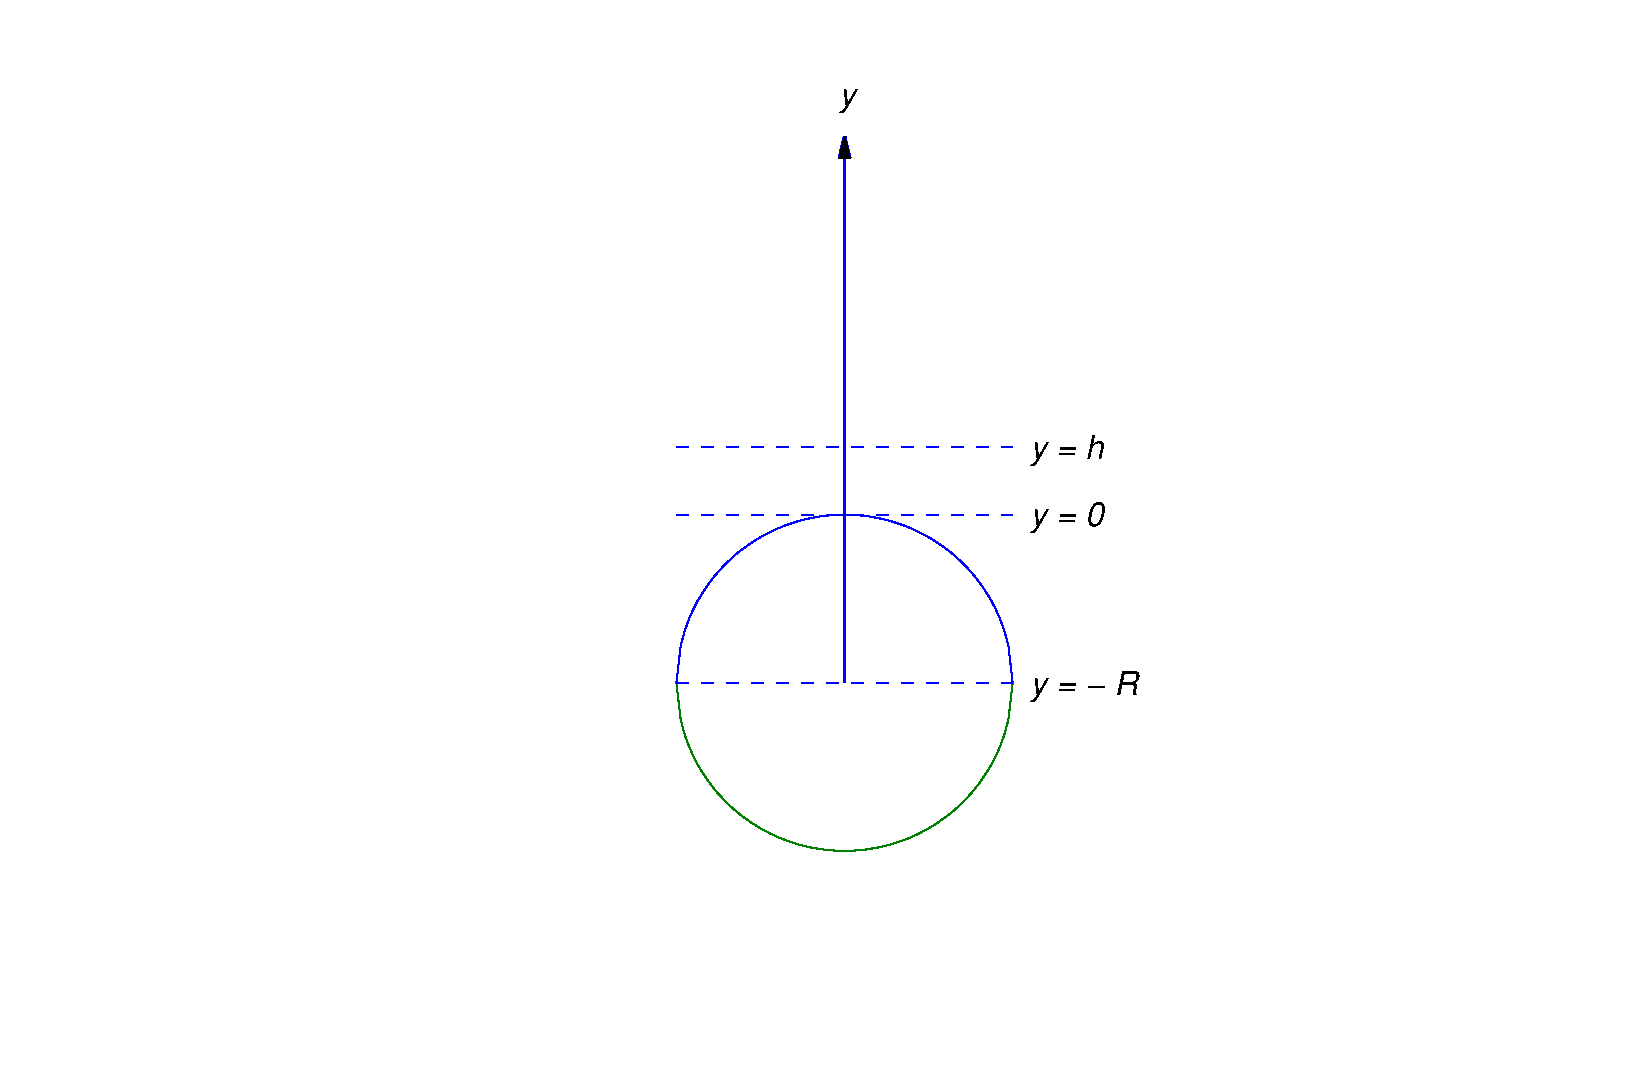
\includegraphics[bb=-78 148 689 643,width=5.67in,height=3.66in,keepaspectratio]{fig040305}
\color{blue}
  \caption{Escape velocity}
  \label{figure:4.3.5}
\end{figure}

 Since $F=-mg$ when $y=0$, setting $y=0$ in
(\ref{eq:4.3.18}) yields
$$
-mg=-{K\over R^2};
$$
 therefore $K=mgR^2$ and (\ref{eq:4.3.18}) can be written more
specifically as
\begin{equation} \label{eq:4.3.19}
F=-{mgR^2\over(y+R)^2}.
\end{equation}

From Newton's second law of motion,
$$
F=m{d^2y\over dt^2},
$$
so (\ref{eq:4.3.19}) implies that
\begin{equation} \label{eq:4.3.20}
{d^2y\over dt^2}=-{gR^2\over(y+R)^2}.
\end{equation}

We'll show that there's a number $v_e$, called the {\color{blue}\it
escape
velocity\/}, with these properties:

\begin{enumerate}
\item If $v_0\ge v_e$ then $v(t)>0$ for all $t>0$, and the vehicle
continues to climb for all $t>0$; that is, it ``escapes'' Earth.
(Is it really so obvious that $\lim_{t\to\infty}y(t)=\infty$
in this case? For a proof, see Exercise~\ref{exer:4.3.20}.)
\item  If $v_0<v_e$  then  $v(t)$   decreases to zero and becomes negative.
Therefore
 the vehicle attains a  maximum
altitude  $y_m$ and
falls back to Earth.
 \end{enumerate}

Since
(\ref{eq:4.3.20}) is second order, we can't solve it by methods discussed
so far. However, we're concerned with $v$ rather than $y$, and $v$ is
easier to find. Since $v=y'$ the chain rule implies that
$$
{d^2y\over dt^2}={dv\over dt}={dv\over dy}{dy\over dt}=v{dv\over dy}.
$$
 Substituting this into (\ref{eq:4.3.20}) yields the first order
separable equation
\begin{equation} \label{eq:4.3.21}
v{dv\over dy}=-{gR^2\over(y+R)^2}.
\end{equation}
When $t=0$, the velocity is $v_0$ and the altitude is $h$. Therefore
we can
obtain $v$ as a function of $y$ by solving the initial value problem
$$
v{dv\over dy}=-{gR^2\over(y+R)^2},\quad  v(h)=v_0.
$$

Integrating (\ref{eq:4.3.21}) with respect to $y$ yields
\begin{equation} \label{eq:4.3.22}
{v^2\over 2}={gR^2\over y+R}+c.
\end{equation}
 Since $v(h)=v_0$,
$$
c={v_0^2\over 2}-{gR^2\over h+R},
$$
 so (\ref{eq:4.3.22}) becomes
\begin{equation} \label{eq:4.3.23}
{v^2\over 2}={gR^2\over y+R}+\left({v_0^2\over 2}-
{gR^2\over h+R}\right).
\end{equation}
If
$$
v_0 \ge\left({2gR^2\over h+R}\right)^{1/2},
$$
 the parenthetical expression in (\ref{eq:4.3.23})  is nonnegative,
 so $v(y)>0$ for $y>h$. This proves that there's an escape
velocity $v_e$. We'll now prove that
$$
v_e=\left({2gR^2\over h+R}\right)^{1/2}
$$
by showing that the vehicle falls back to Earth if
\begin{equation} \label{eq:4.3.24}
v_0 <\left({2gR^2\over h+R}\right)^{1/2}.
\end{equation}
If (\ref{eq:4.3.24})  holds then  the parenthetical expression in
(\ref{eq:4.3.23})
is negative and the vehicle will attain a maximum altitude $y_m>h$
that satisfies the equation
$$
0={gR^2\over y_m+R}+\left({v_0^2\over 2}-
{gR^2\over h+R}\right).
$$
The velocity will be zero at the maximum  altitude, and the object will
then fall to Earth under the influence of gravity.

\exercises
Except where directed otherwise, assume that the magnitude of the
gravitational force on an object with mass $m$ is constant and equal
to $mg$. In exercises involving vertical motion take the upward
direction to be positive.

\begin{exerciselist}

\item\label{exer:4.3.1}
A firefighter  who weighs 192 lb slides down an infinitely long
fire pole
that exerts a frictional resistive force with magnitude proportional
to his speed, with $k=2.5$ lb-s/ft. Assuming that he starts from
rest, find his velocity as a function of time and find his terminal
velocity.

\item\label{exer:4.3.2}
A firefighter who weighs 192 lb slides down an infinitely long
fire pole
that exerts a frictional resistive force with magnitude proportional
to her speed, with constant of proportionality $k$. Find $k$, given
that her terminal velocity is -16 ft/s, and then find her velocity
$v$ as a function of $t$. Assume that she starts from rest.

\item\label{exer:4.3.3}
A boat weighs 64,000 lb. Its propellor produces a constant thrust of
50,000 lb and the water exerts a resistive force with magnitude
proportional to the speed, with $k=2000$ lb-s/ft. Assuming that the
boat starts from rest, find its velocity as a function of time, and
find its terminal velocity.

\item\label{exer:4.3.4}
A constant horizontal force of 10 N pushes a 20 kg-mass through a
medium that resists its motion with .5 N for every m/s of speed. The
initial velocity of the mass is 7 m/s in the direction opposite to
the direction of the applied force. Find the velocity of the mass for
$t > 0$.

\item\label{exer:4.3.5}
A stone weighing 1/2 lb is thrown upward from an initial height of 5
ft with an initial speed of 32 ft/s. Air resistance is
proportional to speed, with $k=1/128$ lb-s/ft. Find the
maximum height attained by the stone.

\item\label{exer:4.3.6}
A 3200-lb car is moving at 64 ft/s down a 30-degree grade when it
runs out of fuel. Find its velocity after that if friction exerts a
resistive force with magnitude proportional to the square of the
speed, with $k=1\ \mbox{lb-s}^2/{\mbox ft}^2$. Also find its
terminal velocity.

\item\label{exer:4.3.7}
A 96 lb weight is dropped from rest in a medium that exerts a
resistive force with magnitude proportional to the speed. Find its
velocity as a function of time if its terminal velocity is -128
ft/s.

\item\label{exer:4.3.8}
An object with mass $m$ moves vertically through a medium that exerts
a resistive force with magnitude proportional to the  speed. Let
$y=y(t)$ be the
altitude of the object at time $t$, with $y(0)=y_0$. Use the results
of Example~\ref{example:4.3.1} to show that
$$
 y(t)=y_0+{m\over k}(v_0-v-gt).
$$

\item\label{exer:4.3.9}
An object with mass $m$ is launched vertically upward with initial
velocity $v_0$ from Earth's surface ($y_0=0$) in a medium that exerts
a resistive force with magnitude proportional to the speed. Find the
time $T$ when the object attains its maximum altitude $y_m$. Then use
the result of Exercise~\ref{exer:4.3.8} to find $y_m$.

\item\label{exer:4.3.10}
An object weighing 256 lb is dropped from rest in a medium that
exerts a resistive force with magnitude proportional to the square of
the speed. The magnitude of the resisting force is 1 lb when $|v|=4\
\mbox{ft/s}$. Find $v$ for $t > 0$, and find its terminal
velocity.

\item\label{exer:4.3.11}
An object with mass $m$ is given an initial velocity $v_0\le0$ in
a medium that exerts
a resistive force with magnitude proportional to the square of the
speed. Find the velocity of the object for $t > 0$, and find its
terminal velocity.

\item\label{exer:4.3.12}
An object with mass $m$ is launched vertically upward with initial
velocity $v_0$ in a medium that exerts a resistive force
with magnitude  proportional to the square of the  speed.

\begin{alist}
\item %(a)
Find the time $T$ when the object reaches its maximum
altitude.
\item %(b)
Use the result of Exercise~\ref{exer:4.3.11} to find the velocity of the
object for $t > T$.
\end{alist}

\item\label{exer:4.3.13} \Lex
An object with mass $m$ is given an  initial velocity $v_0\le0$
in a medium that exerts a resistive force of the form
 $a|v|/(1+|v|)$, where  $a$ is positive constant.

\begin{alist}
\item % (a)
Set up a differential equation for the speed of the object.
\item % (b)
Use your favorite numerical method to solve the equation you found in
\part{a}, to convince yourself that there's  a unique number $a_0$ such
that $\lim_{t\to\infty}s(t)=\infty$ if $a\le a_0$ and
$\lim_{t\to\infty}s(t)$ exists (finite) if $a>a_0$. (We say that $a_0$
is the {\color{blue}\it bifurcation value\/} of $a$.) Try to find $a_0$ and
$\lim_{t\to\infty}s(t)$ in the case where $a>a_0$.
\hint{See Exercise~$\ref{exer:4.3.14}$.}
\end{alist}

\item\label{exer:4.3.14}
An object of mass $m$ falls in a medium that exerts a resistive force
$f=f(s)$, where $s=|v|$ is the speed of the object. Assume that
$f(0)=0$ and $f$ is strictly increasing and differentiable on
$(0,\infty)$.
\begin{alist}
\item % (a)
Write a differential equation for the speed $s=s(t)$ of the object.
Take it as given that all solutions of this equation with $s(0)\ge0$
are defined for all $t>0$ (which makes good sense on physical
grounds).
\item % (b)
Show that if $\lim_{s\to\infty}f(s)\le mg$ then
$\lim_{t\to\infty}s(t)=\infty$.
\item % (c)
Show that if $\lim_{s\to\infty}f(s)>mg$ then
$\lim_{t\to\infty}s(t)=s_T$ (terminal speed), where $f(s_T)=mg$.
\hint{Use Theorem~\ref{thmtype:2.3.1}}.
\end{alist}

\item\label{exer:4.3.15}
A 100-g mass with initial velocity $v_0\le0$ falls in a medium that
exerts a resistive force proportional to the fourth power of the
speed. The resistance is $.1$ N if the speed is 3 m/s.

\begin{alist}
\item % (a)
Set up the initial value problem for the velocity $v$ of the mass for
$t>0$.
\item % (b)
Use Exercise~\ref{exer:4.3.14}(c) to determine the terminal velocity of
the object.
\item % (c)
\Cex
To confirm your answer to \part{b},  use one of the numerical methods  studied
in Chapter~3 to compute  approximate solutions on $[0,1]$
(seconds) of the initial value problem of \part{a}, with initial values
$v_0=0$, $-2$, $-4$, \dots, $-12$. Present your results in graphical form
similar to Figure~\ref{figure:4.3.3}.
\end{alist}

\item\label{exer:4.3.16}
A 64-lb object with initial velocity $v_0\le0$ falls through a dense
fluid that exerts a resistive force proportional to the square root of
the speed. The resistance is $64$ lb if the speed is 16 ft/s.

\begin{alist}
\item % (a)
Set up the initial value problem for the velocity $v$ of the mass for
$t>0$.
\item % (b)
Use Exercise~\ref{exer:4.3.14}(c) to determine the terminal velocity of
the object.
\item % (c)
\Cex
To confirm your answer to \part{b}, use one of the numerical methods
studied in Chapter~3 to compute approximate
solutions on
$[0,4]$ (seconds) of the initial value problem of \part{a}, with
initial values $v_0=0$, $-5$, $-10$, \dots, $-30$. Present your results in
graphical form similar to Figure~\ref{figure:4.3.3}.
\end{alist}

\exercisetext{In Exercises \ref{exer:4.3.17}-\ref{exer:4.3.20}, assume
that the
force due to gravity is given by Newton's law of gravitation. Take the
upward direction to be positive.}

\item\label{exer:4.3.17}
A space probe is to be launched from a space station 200
miles above Earth.  Determine its escape velocity in
miles/s.  Take Earth's radius to be 3960 miles.

\item\label{exer:4.3.18}
A space vehicle is to be launched from the moon, which has a
radius of about 1080 miles.  The acceleration due to
gravity at the surface of the moon is about $5.31$
ft/s$^2$.  Find the escape velocity in miles/s.

\item\label{exer:4.3.19}
\begin{alist}
\item %(a)
Show that Eqn.~(\ref{eq:4.3.23})  can be rewritten as
$$
v^2={h-y\over y+R} v^2_e+v_0^2.
$$
\item %(b)
Show that if $v_0=\rho v_e$ with $ 0\le \rho < 1$, then
the maximum altitude $y_m$ attained by the space
vehicle is
$$
y_m={h+R\rho^2\over 1-\rho^2}.
$$
\item %(c)
By requiring that $v(y_m)=0$, use Eqn.~(\ref{eq:4.3.22}) to
deduce that if $v_0 < v_e$ then
$$
|v|=v_e\left[{(1-\rho^2)(y_m-y)\over y+R}\right]^{1/2},
$$
where $y_m$ and $\rho$ are as defined in \part{b} and
$y \ge h$.
\item %(d)
Deduce from \part{c} that if $v < v_e$,  the vehicle takes
equal times to climb from $y=h$ to $y=y_m$ and to
fall back from $y=y_m$ to $y=h$.
\end{alist}

\item\label{exer:4.3.20}
In the situation considered in the discussion of escape velocity, show
that $\lim_{t\to\infty}y(t)=\infty$ if $v(t)>0$ for all $t>0$.

\hint{Use a proof by contradiction. Assume that there's a number
$y_m$ such that $y(t)\le y_m$ for all $t>0$. Deduce from this that
there's positive number $\alpha$ such that $y''(t)\le-\alpha$ for all
$t\ge0$. Show that this contradicts the assumption that $v(t)>0$ for
all $t>0$.}
\end{exerciselist}
